\newpage
\section{Лекция 7}
\subsection{Матричные нормы}
\begin{definition}
    Рассмотрим линейное пространство матриц размера $n$ над комплексными числами. Норма $||\cdot||$ на пространстве $V=M_{n\times n}(\mathbb{C})$ называется \textbf{матричной нормой}, если \begin{enumerate}[start=0]
        \item Это норма.
        \item Норма $||\cdot ||$ является \textbf{согласованной с операцией умножения}, то есть $$||AB|| \leq ||A|| \; ||B|| \text{ для любых } A, B \in M_{n\times n}(\mathbb{C}),$$ (удовлетворяет свойству субмультипликативности).\end{enumerate}
\end{definition}
\begin{lemma}[Свойства]
    \ 
    \begin{enumerate}
        \item  $||E||\geqslant1$\\
        $\blacktriangleright ||E||\leqslant||E||~||E|| \Rightarrow ||E||\geqslant1~~\blacksquare$
        \item Матричная норма называется \textbf{сохраняющей единицу}, если $||E||=1.$
        \item Матричная норма называется \textbf{согласованной с векторной нормой} $|\cdot|$ на $\mathbb{C}^n$, если $$|M\bar x|\leqslant||M||\cdot |\bar x|.$$
        \item Если $||M||$ --- матричная норма, тогда $||M||_*=||M||x,~x\geqslant1$ --- тоже матричная норма.
    \end{enumerate}
\end{lemma}
\textbf{Примеры матричных норм.}
\begin{itemize}
    \item \textbf{$||M||=\sum\limits_{i, j=1,...,n}|m_{ij}|$}\\
    $M=(m_{ij})_{n\times n}$\\
    Проверим свойства:\begin{enumerate}[start=0]
        \item Это норма Гельдера $|\cdot |_1$ на $\mathbb{C}^{n^2}$.
        \item $||M||=|M^1|_1+\cdots|M^n|_1$\\
        $||AB||=\sum\limits_{i,j}|\sum\limits_t a_{it}b_{tj}|\leqslant \sum\limits_{i,j,t}|a_{it}||b_{tj}|\leqslant \sum\limits_{i,j,t,s}|a_{i,s}||b_{tj}|=\sum\limits_{i,s}|a_{is}|\sum\limits_{t, j}|b_{tj}|\leqslant||A||\cdot||B||$
        \item $||E||=n$ --- не выполняется, не сохраняет единицу.\\
        \item \begin{itemize}
            \item Согласована ли с $|\cdot|_1$ ?\\
            $$|Mx|_1 \overset{?}{\leqslant} ||M||\cdot |x|_1$$
            \[|Mx|_1 = \Bigg | \Bigg | M\cdot \Bigg( \bar x \begin{pmatrix}[c]
            0 & \vline~ \cdots~ \vline& 0\\ 
            \vdots & \vline~ \cdots ~\vline& \vdots\\
            0 & \vline~ \cdots ~\vline& 0
            \end{pmatrix}\Bigg) \Bigg | \Bigg |, ~ |x|_1 = ||B||\]\\
            То есть, согласована.
            \item Согласована с $|\cdot|_\infty$ ? 
            \[M_{n \times n} = \begin{pmatrix}
            M_1\\
            \vdots\\
            M_n
            \end{pmatrix}, ~Mx=\begin{pmatrix}
            M_1x\\
            \vdots\\
            M_nx
            \end{pmatrix}\]\begin{center}
                $|Mx|=max|<M_i, \bar x>| \leqslant |x_{max}|\sum\limits_{i,j}^n|m_{ij}|\leqslant |x|_{\infty}||M||$\end{center}
            То есть, согласована.
        \end{itemize}
    \end{enumerate}
    \item \textbf{Норма Фробениуса $||M||_F=\sqrt{\sum\limits_{i,j}|m_{ij}|^2}$}\\
    0. Это Евклидова норма на пространстве.\\
    1. $||M||_F^2=tr(M^*M)=\sum\limits_{i=1}^n\lambda_i(M^*M)=\sigma_1^2+\cdots+\sigma_n^2$ --- сумма квадратов сингулярных значений (согласованность с умножением).\\
    Если $U$ --- унитарная матрица, например, поворот, то есть, $U^*=U^{-1}$, то $$||U^{-1}MU||_F^2=tr((U^*MU)^*U^*MU)=tr(U^*M^*MU)=tr(M^*M)=||M||_F^2$$
    Более того: $||UM||_F=tr(M^*U^*UM)=tr(M^*M)=||M||_F^2$.\\
    $M=U\Sigma V^*,~U$ и $V$ --- ортогональные\\
    \[\Sigma = \begin{pmatrix}
    \sigma_1 & \cdots & 0\\
    \vdots & \ddots & \vdots\\
    0 & \cdots \sigma_n
    \end{pmatrix}\]
    $$||M||=||\Sigma||$$
    Норма Фробениуса $||M||_F$ согласована с евклидовой $|\bar x|_2$.
\end{itemize}
\subsection{Индуцированные нормы}
\begin{definition}
    Пусть на $\mathbb{C}^n$ задана норма $|\cdot |_1$. Функция из $M_n$ в $\mathbb{C}$: $||M||=\underset{x\neq 0}{max} \cfrac{|Mx|}{|x|}$ называется \textbf{матричной нормой, индуцированной векторной нормой} $|\cdot|$.
\end{definition}
Если $c=|x|$, $y=\cfrac{x}{|x|}$, $|y|=1$, то $Mx=M(cy)=cMy.$ А так как $c>0$, то $|Mx|=c|My|$.\\
То есть, здесь максимум достигается, так как: $$\underset{x\neq y}{max}\cfrac{|Mx|}{|x|}=\underset{|y|=1}{max}\cfrac{c|My|}{c}=\underset{|y|=1}{max}|My|=\underset{y\in B_1}{max}|My|$$.\begin{center}
    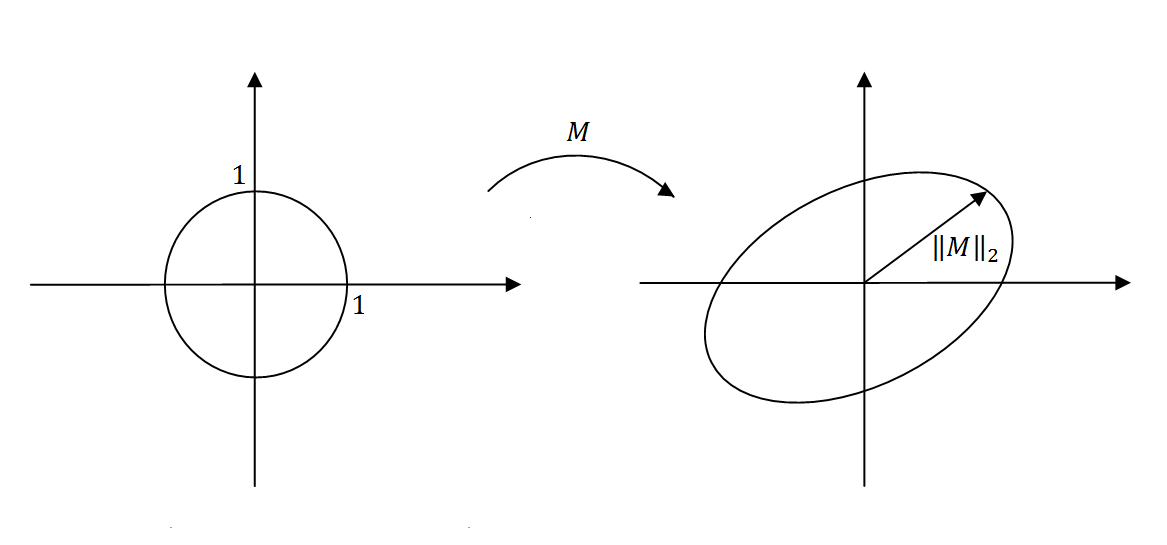
\includegraphics[scale=0.6]{l7_1.png}\end{center}
\begin{theorem}
    Пусть $||\cdot ||_{\star}$ индуцирована $|\cdot |_{\star}$, тогда
    \begin{enumerate}
        \item $||\cdot ||$ --- матричная норма, выполнены свойства 0, 1
        \item $||\cdot ||_{\star}$ согласована с $|\cdot |_{\star}$
        \item $||\cdot ||_{\star}$ сохраняет единицу
        \item Если существует другая норма $||\cdot ||$, согласованная с $||\cdot||_{\star}$, то $||M|| \geqslant ||M||_{\star}$ ($||M_{\star}||$ минимальна).
    \end{enumerate}
\end{theorem}
\begin{proof}
    \ 
    \begin{enumerate}
    \item Очевидно.
    \item $ |Mx|_{\star}\underset{x\neq \bar 0}{=}\cfrac{|Mx|_{\star}}{|x|_{\star}}|x|_{\star} \leqslant \underset{z}{max}\cfrac{|Mz|_{\star}}{|z|_{\star}}|x|_{\star}=||M||_{\star}|x|_{\star}$
    \item $ ||E||_{\star}=\underset{|y|_{\star}=1}{max}|Ey|_{\star}=\underset{|y|_{\star}=1}{max}|y|_{\star}=1$ 
    \item Пусть $|y|_{\star}=1$ и $||M||_{\star}=|My|_{\star}$, тогда длина матрицы $||M||_{\star}=|My|_{\star} \leqslant ||M||\cdot |y|_{\star}=||M||$
\end{enumerate}
\end{proof}
\begin{theorem}
    \ 
\begin{center}
    \begin{tabular}{ | c || c |}
        \hline
        Векторная норма $|\cdot|_{\star}$ & Индуцированная норма $||\cdot||_{\star}$\\ \hline \hline
        $||\bar x||_1 = \sum\limits_{i=1}^n |x_i|$ & $||M||_1 = \underset{j}{max}|M^j|_1=\underset{j}{max}\sum\limits_i|m_{ij}|=||M^*||_1$  \\ \hline \hline
        $||\bar x||_2  = \sqrt{\sum\limits_{i=1}^n |x_i|^2}$ & $\sigma(M)=\sqrt{max \lambda_{M^*M}}$ (сингулярный радиус матрицы) \\
        \hline \hline
        $||\bar x||_\infty = \underset{1\leq i \leq n}{max} |x_i|$ & $||M||_{\infty} = \underset{i}{max}|M_i|_1=\underset{i}{max}\sum\limits_j|m_{ij}|$ \\ \hline
    \end{tabular}
\end{center}
\end{theorem}
\begin{proof}
Докажем, что векторной норме $|\bar x|_1$ соответствует индуцированная матричная норма $||M||_1$.\\
\begin{center} $M=(M^1,\cdots, M^n)$\\
    $Mx+M^1x_1+\cdots M^nx_n$\\
    $|Mx|_1\leqslant |M^1x_1+\cdots+M^nx_n|_1\leqslant|x_1|~|M^1|_1+\cdots+|M^n|_1~|x_n|\leqslant(|x_1|+\cdots+|x_n|)\underset{j}{max}|M^j|_1\leqslant|\bar x|_1\underset{j}{max}|M^j|_1$\end{center}
Пусть максимум достигается на первом столбце, тогда $|Mx|_1=\sum\limits_{j=1}^n|m_{1j}|=||M||_1$.\\
Оценка достигается, значит это и есть максимум.
\end{proof}
\subsection{Домашнее задание 7}
\begin{enumerate}
    \item Доказать, что векторной норме $|\bar x|_2$ соответствует индуцированная матричная норма $\sigma(M)$.
    \item Доказать, что векторной норме $|\bar x|_{\infty}$ соответствует индуцированная матричная норма $||M||_{\infty}$.
    \item Является ли матричной нормой $f(A)=\underset{1\leqslant i,~j\leqslant n}{max}|a_{ij}|$ ?
    \item Доказать $||A^{-1}||\geqslant\cfrac{||E||}{||A||}.$
    \item Найти все нормы: $||A||_{\infty}, ~||A||_1, ~\sigma(A)$ для матрицы \[\begin{pmatrix}
    1 & 2 & 3\\
    4 & 5 & 6\\
    7 & 8 & 9
    \end{pmatrix}\]
    \item Найти $x,~y,~z,~t$ для матрицы $A$ \[A=\begin{pmatrix}
    1 & 2\\
    3 & 4
    \end{pmatrix}\]
    \begin{center}
        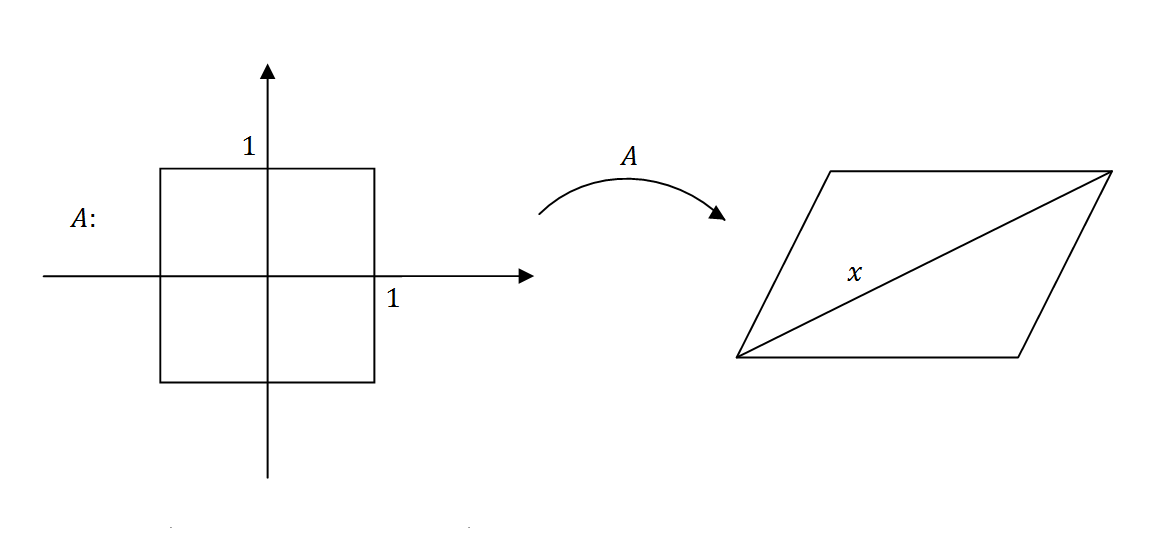
\includegraphics[scale=0.6]{l7_2.png}\\
        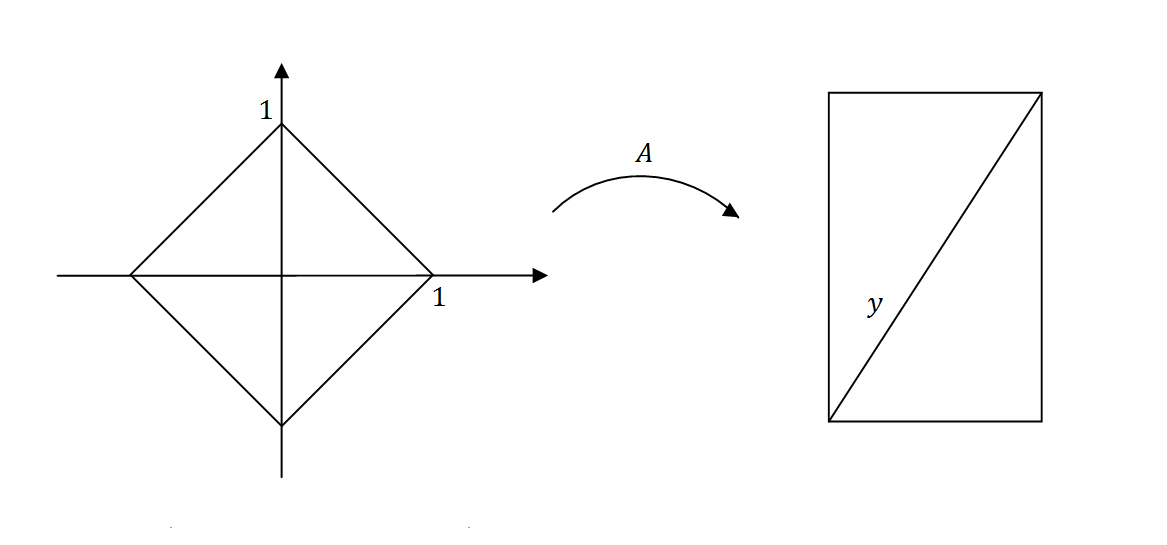
\includegraphics[scale=0.6]{l7_3.png}\\
        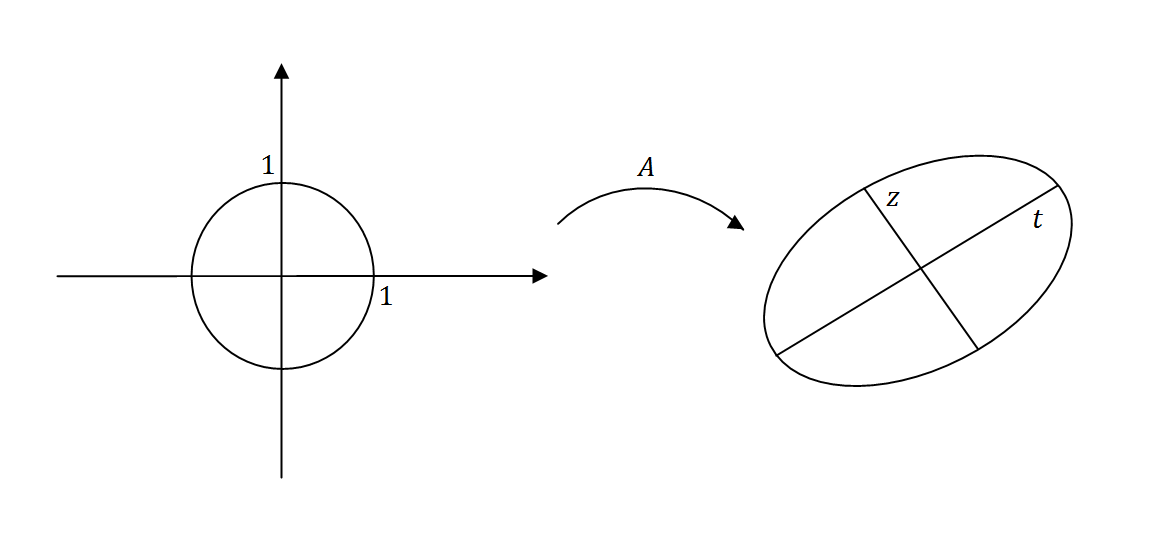
\includegraphics[scale=0.6]{l7_4.png}
    \end{center}
\end{enumerate}